
\section{Results}

This section presents the numerical assessment of both, the primal and dual formulation presented above. We consider two numerical examples. The first one aims to assess the convergence properties of the methods by computing the errors with respect to a smooth manufactured solution. The results are also compared with the Natural, Equal-Order Fully Stabilized, and Equal-Order Unstabilized formulations recently presented in \cite{ddcm1_article_gus}. 
The second example considers a more challenging problem that exhibits an internal reaction
boundary layer, so as to assess the approximation properties of the proposed methods in the presence
of large gradients. This example nicely illustrates some key differences between the primal
and the dual formulations and also allows us to study the effect of different choices for the data 
fields $(\eFt,\sFt)$, which is more appealing in data-driven computational mechanics computations.

We consider a sequence of conforming and shape-regular finite element partitions of the computational domain, denoted by $\mathcal{T}_h$, with characteristic mesh size $h$. 
One of the main motivations of the variational multiscale approach is the possibility of equal-order approximations.
Therefore we consider the following choice of discrete finite element spaces 
\begin{equation*}\label{eq:equal_order_func_spaces}
	\left(\uF_{h}, \eF_{h}, \sF_{h}, \lF_{h}, \mF_{h}\right)
	\in
	\CG_{k} \times \left[\CG_{k}\right]^{d_{\Omega}}
	\times \left[\CG_{k}\right]^{d_{\Omega}}
	\times \CG_{k}
	\times \left[\CG_{k}\right]^{d_{\Omega}},
\end{equation*}
where $d_{\Omega}$ denotes the spatial dimension of the computational domain $\Omega$, $k>0$ and 
\begin{equation*}
	\quad \CG_{k} := \left\{ v \in C^0(\Omega) \;\middle|\; v|_K \in \mathbb{P}_k(K),\ \forall K \in \mathcal{T}_h \right\}	
\end{equation*}
where $\mathbb{P}_k(K)$ denotes the space of polynomials of degree $k$ defined on each element $K \in \mathcal{T}_h$.
A comment is in order to as the computation of the subscale component of the discrete solution. 
Whereas in the ASGS method, being $P'$ the identity operator, no additional unknowns are 
needed, since the subscales are simply evaluated locally at the element level, for the OSS 
method, with $P'$ being the projector onto the orthogonal complement of the finite element space, 
we need to introduce one additional unknown for each field if we aim to solve the problem monolithically,
this is, if we denote by $w$ any field, such that $w = w_h + w'$, $w'$ is given by
\begin{equation}
w' = \tau_w \ P' \left ( r(w) \right ) = r(w) - P_{L^2(\Omega)} \left ( r(w) \right )
\end{equation}



Although it is worth mentioning at this point that no significative differences were observed between the two approaches in both, the primal and dual formulations. 

Finally, the implementation was done in the finite element platform Firedrake \cite{firedrake} and is available in \cite{githubrepoddcm}.

\newpage
\subsubsection{Convergence to a manufactured solution}

First, we define the parameters employed in each formulation. For this purpose, we consider $P'$ to be the identity operator in both the primal and dual problems. Accordingly, we shall hereafter refer to these formulations as \textbf{Primal-ASGS} and \textbf{Dual-ASGS}. Additionally, the stabilization constants for the primal formulation are chosen as
$$
k_{\uF} = k_{\lF} = 0, 
\quad 
k_{\eF} = k_{\sF} = k_{\mF} = \tfrac{1}{8},
$$
whereas for the dual formulation we take
$$
k_{\uF} = k_{\lF} = k_{\eF} = k_{\mF} = \tfrac{1}{4}, 
\quad 
k_{\sF} = 1.0.
$$
%\quad  k_{\mF} = \tfrac{1}{8}. 
The former choice exploits the residual orthogonality property proved earlier, while the latter ensures that $k_{\eF}$ can be chosen independently of the mesh size. Moreover, the characteristic length scale of the problem is fixed as $\ell = 1$, which implies $L_{0} \sim h$ and $L_{1} \sim \tfrac{1}{h}$ for the $P_{p,h}$, whereas $L_{0} \sim 1$ and $L_{1} \sim 1$ for $P_{d,h}$. As a final remark, in the convergence studies presented below we consider linear and quadratic polynomial approximations, corresponding to degrees $k \in \{0,1\}$.

Now we describe the construction of the manufactured solution employed in this test problem. Although it is essentially the same as that adopted for the convergence assessment in a convex domain in \cite{X}, we opted to give a brief review. Let $\uF$ denote the smooth scalar field defined by
\begin{equation}
	\uF : \Omega \to \mathbb{R}, \qquad \uF(x,y) = \cos(\pi x)\cos(\pi y),
\end{equation}
whose gradient is given by
\begin{equation}
	\eF : \Omega \to \mathbb{R}^{2}, \qquad 
	\eF(x,y) = -\pi \,[\sin(\pi x)\cos(\pi y),\, \cos(\pi x)\sin(\pi y)]^{\top}.
\end{equation}
Then, we propose $\lambda$ to be as
\begin{equation}
	\lF : \Omega \to \mathbb{R}, \qquad 
	\lF(x,y) = -\frac{1}{40\pi}\,[\cos(2\pi x) + \cos(2\pi y)],
\end{equation}
and define $\sF$ as follows
\begin{equation}\label{eq:nonlinear_fluxlaw}
	\sF : \Omega \to \mathbb{R}^{2}, \qquad 
	\sF = -\frac{\eF}{\|\eF\|}\left(\|\eF\| - \frac{1}{40}\,\|\eF\|^{3}\right).
\end{equation}
This way, eq.~\ref{eq:nonlinear_fluxlaw} establishes a nonlinear constitutive relation between flux $\sF$ and gradient $\eF$. 

Similarly to the approach in \cite{X}, and solely for the purpose of assessing the convergence properties of the discrete formulations under general conditions, it is convenient to add an additional source term to the right-hand side of eqs.~\ref{X} and \ref{X}:
\begin{equation}
	\zeta \lF + \nabla \cdot \mF = f,
\end{equation}
which amounts to adding the term \(- (f, \uF)\) to the Lagrangian (eq.~\ref{X}).

By examining the optimality conditions in their strong form either from $P_{p,h}$ or $P_{d,h}$ (eqs.~\ref{X} and \ref{X} respectively), we proceed as follows to construct the manufactured solution for the remaining fields. First take
\begin{equation}
	\eFt:\Omega \rightarrow \mathbb{R}^2, \qquad \eFt(x,y) = \eF(x,y) + \frac{1}{20} \left[\sin\left(4\,\pi\,x \right), \sin\left(4\,\pi\,y\right) \right]^{\top}
\end{equation}
as a perturbation of $\eF$, from which $\mF$ can be obtained using the last optimality condition. Then, $\sFt$ is computed from the third optimality condition, and finally, the source terms $f$ and $q$ are determined by substituting the proposed fields into the first and second equations.

In the numerical experiment, the computational domain $\Omega$ is chosen to be the unit square $[0,1]^2$. On the boundary $\partial \Omega$, we impose pure Dirichlet boundary conditions, i.e.,
\begin{equation}
	\left\lbrace
	\begin{array}{rclll}
		\uF &=& \mathsf{g}_{\uF} &\mbox{on}&~\partial \Omega, \\
		\lF &=& \mathsf{g}_{\lF} &\mbox{on}&~\partial \Omega, \\
	\end{array}
	\right.
\end{equation}
where the values on the right-hand side are computed from the manufactured fields. Finally, the diffusion and reaction coefficients are taken as unity, i.e., $\kappa = 1$ and $\zeta = 1$.

%=============================================
% k = 0

\begin{figure}[h!]
	\centering
	\caption{Convergence of scalar fields $\uF$ and $\lF$ for $k = 0$. Figures (a)--(b) show the results for $\uF$, and (c)--(d) for $\lF$, considering all formulations: Natural, Equal-Order Unstabilized, Equal-Order Fully Stabilized, Primal-ASGS, and Dual-ASGS. Errors are evaluated in the $L^2$ and $H^1$ norms, as indicated. For the Dual-ASGS formulation, only the $L^2$ norm is assessed.}
	%\fontsize{11pt}{10pt}\selectfont 
	\def\svgwidth{1.0\columnwidth}
	\input{Figures/PDFs/convergence_scalar_linear_art02.pdf_tex}
	\label{fig:convergence_scalar_linear_art02}
\end{figure}


\begin{figure}[h!]
	\centering
	\caption{Convergence of vector fields $\sF$, $\eF$, and $\mF$ with $k=0$, evaluated in the $L^{2}$-norm considering all formulations: Natural, Equal-Order Unstabilized, Order-Order Fully Stabilized, Primal-ASGS, and Dual-ASGS.
	}
	%\fontsize{11pt}{10pt}\selectfont 
	\def\svgwidth{1.0\columnwidth}
	\input{Figures/PDFs/convergence_vector_linear_art02.pdf_tex}
	\label{fig:convergence_vector_linear_art02}
\end{figure}


\begin{figure}[h!]
	\centering
	\caption{Convergence of vector fields $\sF$, $\eF$, and $\mF$ with $k=0$, evaluated in the Hdiv-norm for Equal-Order Unstabilized, Equal-Order Fully Stabilized, Primal-ASGS, and Dual-ASGS formulations.
	}
	%\fontsize{11pt}{10pt}\selectfont 
	\def\svgwidth{1.0\columnwidth}
	\input{Figures/PDFs/convergence_vector_linear_hdiv_art02.pdf_tex}
	\label{fig:convergence_vector_linear_hdiv_art02}
\end{figure}


%=============================================
% k = 1

\begin{figure}[h!]
	\centering
	\caption{Convergence of scalar fields $\uF$ and $\lF$ for $k = 1$. Figures (a)--(b) show the results for $\uF$, and (c)--(d) for $\lF$, considering all formulations: Natural, Equal-Order Unstabilized, Equal-Order Fully Stabilized, Primal-ASGS, and Dual-ASGS. Errors are evaluated in the $L^2$ and $H^1$ norms, as indicated. For the Dual-ASGS formulation, only the $L^2$ norm is assessed.}
	%\fontsize{11pt}{10pt}\selectfont 
	\def\svgwidth{1.0\columnwidth}
	\input{Figures/PDFs/convergence_scalar_quadratic_art02.pdf_tex}
	\label{fig:convergence_scalar_quadratic_art02}
\end{figure}


\begin{figure}[h!]
	\centering
	\caption{Convergence of vector fields $\sF$, $\eF$, and $\mF$ with $k=1$, evaluated in the $L^{2}$-norm considering all formulations: Natural, Equal-Order Unstabilized, Equal-Order Fully Stabilized, Primal-ASGS, and Dual-ASGS.}
	%\fontsize{11pt}{10pt}\selectfont 
	\def\svgwidth{1.0\columnwidth}
	\input{Figures/PDFs/convergence_vector_quadratic_art02.pdf_tex}
	\label{fig:convergence_vector_quadratic_art02}
\end{figure}

\begin{figure}[h!]
	\centering
	\caption{Convergence of vector fields $\sF$, $\eF$, and $\mF$ with $k=1$, evaluated in the Hdiv-norm for Equal-Order Unstabilized, Equal-Order Fully Stabilized, Primal-ASGS, and Dual-ASGS formulations.}
	%\fontsize{11pt}{10pt}\selectfont 
	\def\svgwidth{1.0\columnwidth}
	\input{Figures/PDFs/convergence_vector_quadratic_hdiv_art02.pdf_tex}
	\label{fig:convergence_vector_quadratic_hdiv_art02}
\end{figure}







\iffalse

\cleardoublepage
\subsubsection{Convergence: a non-convex domain}
With reference to the non-convex domain discussed in \cite{X}, we now assess the accuracy of both \textbf{Primal-ASGS} and \textbf{Dual-ASGS} formulations for the re-entrant corner problem, whose geometry is shown in Fig.~\ref{X} for the opening angle $\phi = \pi/4$. The corner is located at the origin $(0,0)$. A manufactured solution is prescribed by defining the scalar field $\uF$ as
\begin{equation*}
	\begin{aligned}
		&\uF: \Omega \rightarrow \mathbb{R}, \quad \uF(x,y) = r^{\nu}\,\sin(\nu\,\theta), \\
		&\text{where} \quad r = \sqrt{x^{2} + y^{2}}, \quad \theta = \arctan{\left(\frac{y}{x}\right)}, \quad \nu = \frac{\pi}{\psi}, \quad \text{and} \quad \psi = 2\pi - \phi.
	\end{aligned}
\end{equation*}
The corresponding gradient field is then given by
\begin{equation*}
	\eF: \Omega \rightarrow \mathbb{R}^{2}, \quad 
	\eF(x,y) = \nu\,r^{\nu-2}
	\begin{bmatrix}
		x\,\sin(\nu\,\theta) - y\,\cos(\nu\,\theta) \\
		y\,\sin(\nu\,\theta) + x\,\cos(\nu\,\theta)
	\end{bmatrix}.
\end{equation*}
By proposing $ \lF $ and $ \eFt $ as in eqs.~(\ref{X}) and~(\ref{X}), respectively, and assuming a linear constitutive flux law, i.e., $ \sF = -\kappa \eF $, the remaining fields can be fully determined. Lastly, it is worth mentioning that pure Dirichlet boundary conditions are imposed for both $\uF$ and $\lF$, prescribed according to the manufactured solution.

\begin{figure}[h!]
	\centering
	\caption{$\uF$ and $\sF$ for the reentrant corner considering both Primal-ASGS and Dual-ASGS formulations.}
	%\fontsize{11pt}{10pt}\selectfont 
	\def\svgwidth{0.8\columnwidth}
	\input{Figures/PDFs/reentrant_u_s_art02.pdf_tex}
	\label{fig:reentrant_u_s_art02}
\end{figure}

\begin{figure}[h!]
	\centering
	\caption{$\lF$ and $\mF$ for the reentrant corner considering both Primal-ASGS and Dual-ASGS formulations.}
	%\fontsize{11pt}{10pt}\selectfont 
	\def\svgwidth{0.8\linewidth}
	\input{Figures/PDFs/reentrant_lam_mu_art02.pdf_tex}
	\label{fig:reentrant_lam_mu_art02}
\end{figure}

\begin{figure}[h!]
	\centering
	\caption{$\uF$, $\sF$, $\lF$ and $\mF$ along the coordinate diagonal for the reentrant corner considering both Primal-ASGS and Dual-ASGS formulations.}
	%\fontsize{11pt}{10pt}\selectfont 
	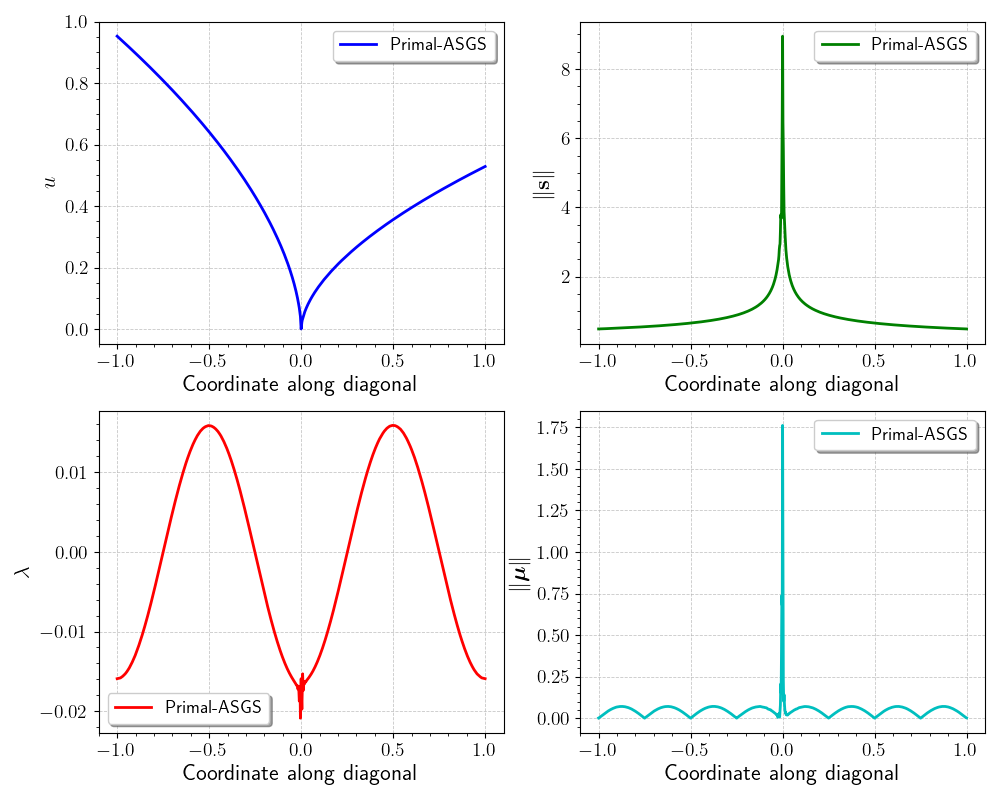
\includegraphics[width=\linewidth]{Figures/PDFs/plot_over_line_reentrant_corner.png}
	\label{fig:}
\end{figure}


\cleardoublepage
\subsubsection{Eigenvalue problems}
To assess the stability of a given finite element discretization, one may consider 
the generalized eigenvalue problem associated with the Babuška–Brezzi conditions. 
Following \cite{X,X}, the Babuška inf–sup constant can be characterized in terms of the 
smallest (in modulus) eigenvalue of a generalized eigenvalue problem.

Let $Z_h = X_h \times Y_h$ denote an abstract discrete mixed function space, on which we 
pose the abstract mixed variational problem: Find $(x_h,y_h) \in Z_h$ such that
\begin{equation*}
	B((x_h,y_h),(\delta x_h, \delta y_h)) = L((\delta x_h, \delta y_h)),
	\qquad \forall\, (\delta x_h, \delta y_h) \in Z_h.
\end{equation*}  
The stability of this discretization is governed by the Babuška inf-sup constant $\gamma_h$, defined as
\[
\gamma_h := \inf_{(x_h,y_h) \in Z_h \setminus \{0\}} \sup_{(\delta x_h, \delta y_h) \in Z_h \setminus \{0\}} \frac{B((x_h,y_h),(\delta x_h, \delta y_h))}{\|(x_h,y_h)\|_{Z_h} \|(\delta x_h, \delta y_h)\|_{Z_h}},
\]
where $\|(x_h,y_h)\|_{Z_h}^2 = \|x_h\|_{X_h}^2 + \|y_h\|_{Y_h}^2$ is the natural norm on the product space.This constant can be characterized by the following generalized eigenvalue problem: Find $0 \neq (x_h,y_h) \in Z_h$ and $\lambda \in \mathbb{R}$ such that
\begin{equation}
	B((x_h,y_h),(\delta x_h, \delta y_h))
	= \lambda \, \left( \langle x_h, \delta x_h \rangle_{X_h}
	+ \langle y_h, \delta y_h \rangle_{Y_h} \right),
	\quad \forall\, (\delta x_h, \delta y_h) \in Z_h.
	\label{eq:babuska-eigen}
\end{equation}
This way, provided the inner product on the right-hand side induces the norm $\|\cdot\|_{Z_h}$ used in the definition of $\gamma_h$, the inf-sup constant is equal to the smallest eigenvalue of this problem in modulus, that is,
\begin{equation}
	\gamma_h = \min_{\lambda \in \sigma(B)} |\lambda|,
\end{equation}
where $\sigma(B)$ denotes the spectrum of the generalized eigenvalue problem.

For the discrete primal formulation $\Pph$, we set $B \leftarrow \Bsp$ and $(x_h,y_h) \leftarrow (\xFh, \varxFh)$; thus the corresponding Babuška eigenvalue problem reads: 
Find $\,0 \neq \xFh= (\uFh,\eFh,\sFh,\lFh,\mFh) \in \XSph$ and $\lambda \in \mathbb{R}$ such that
\begin{equation}
	\Bsp(\xFh,\varxF)
	= \lambda\, (\xFh,\varxF)_{\XSph},
	\qquad \forall\, \varxFh \in \XSph,
	\label{eq:primal-babuska-eigen}
\end{equation}
where $(\cdot,\cdot)_{\XSph}$ denotes the inner product inducing the norm 
$\|\cdot\|_{\XSph}$ defined in Section~\ref{sec:X}. Similarly, for the discrete dual problem $\Pdh$, we set $B \leftarrow \Bsd$ and $(x_h,y_h) \leftarrow (\xFh, \varxFh)$; thus the corresponding Babuška eigenvalue problem reads: 
Find $\,0 \neq \mathbf{x}_h = (\uFh,\eFh,\sFh,\lFh,\mFh) \in \XSdh$ and $\lambda \in \mathbb{R}$ such that 
\begin{equation}
	\Bsd(\xFh,\varxFh)
	= \lambda\, (\xFh,\varxFh)_{\XSdh},
	\qquad \forall\, \varxFh \in \XSdh,
	\label{eq:dual-babuska-eigen}
\end{equation}
where $(\cdot,\cdot)_{\XSdh}$ denotes the inner product inducing the norm $\|\cdot\|_{\XSdh}$ defined in Section~\ref{sec:X}.
In both cases, the discrete eigenvalue problem admits the following algebraic representation:
\begin{equation}
	\mathbf{A}\,\mathbf{x} = \lambda\,\mathbf{M}\,\mathbf{x},
	\label{eq:babuska-matrix}
\end{equation}
with $\mathbf{A}_{p}$ (resp.~$\mathbf{A}_{d}$) and $\mathbf{M}_{p}$ (resp.~$\mathbf{M}_{d}$)
are the matrices associated, respectively, with the stabilized bilinear forms
$\Bsp$ (resp.~$\Bsd$) and the inner products
$(\cdot,\cdot)_{\XSph}$ (resp.~$(\cdot,\cdot)_{\XSdh}$).

Having established the eigenvalues problems for both discrete primal and dual problems, we shall present that $\gamma_{h,p}$ and $\gamma_{h,d}$ (associated to the primal and dual problems) are bounded from below independently of $h$. 



\fi






